\chapter{Experiment s dlhou trasou a dlhým vozidlom}\label{longDlongV}

\begin{figure}[h]
  \centering
  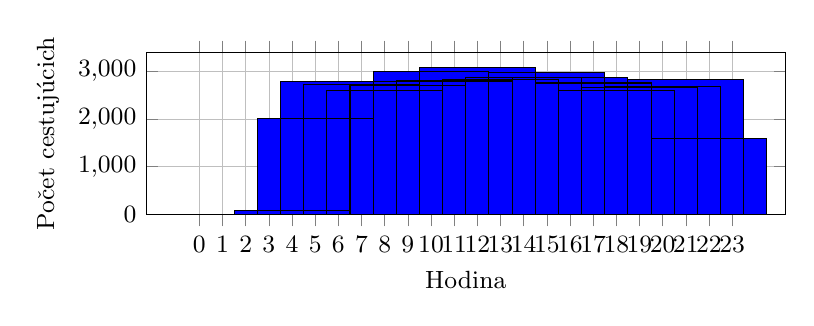
\begin{tikzpicture}
    \begin{axis}[
      width=0.8\textwidth,
      height=0.3\textwidth,
      xlabel={Hodina},
      ylabel={Počet cestujúcich},
      ymin=0,
      xtick={0,1,...,23},
      grid=both,
      major grid style={line width=.2pt,draw=gray!50},
      minor grid style={line width=.1pt,draw=gray!20},
      tick label style={font=\small},
      label style={font=\small},
      legend style={font=\small, at={(0.5,-0.2)}, anchor=north, legend columns=-1},
      ybar,
      bar width=5,
      ]
      \addplot[fill=blue] coordinates {
        (0, 0) (1, 0) (2, 0) (3, 0) (4, 88) (5, 2011) (6, 2784) (7, 2716) 
        (8, 2584) (9, 2696) (10, 2996) (11, 2792) (12, 3079) (13, 2832) 
        (14, 2866) (15, 2964) (16, 2857) (17, 2749) (18, 2587) (19, 2659) 
        (20, 2683) (21, 2823) (22, 1592) (23, 0)
      };
    \end{axis}
  \end{tikzpicture}
  \caption{Počet cestujúcich prichádzajúcich na zastávku za hodinu}
\end{figure}

\begin{figure}[h]
  \centering
  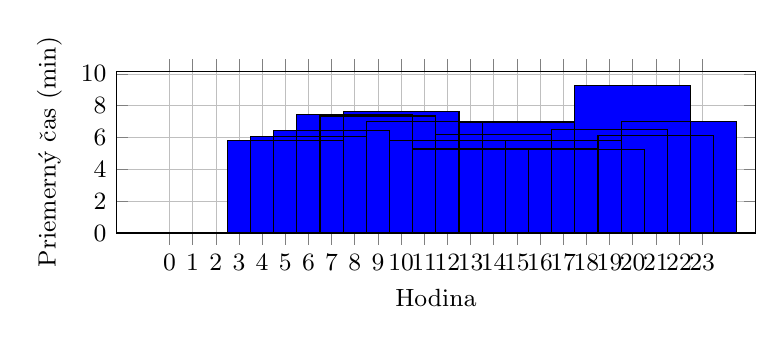
\begin{tikzpicture}
    \begin{axis}[
      width=0.8\textwidth,
      height=0.3\textwidth,
      xlabel={Hodina},
      ylabel={Priemerný čas (min)},
      ymin=0,
      xtick={0,1,...,23},
      grid=both,
      major grid style={line width=.2pt,draw=gray!50},
      minor grid style={line width=.1pt,draw=gray!20},
      tick label style={font=\small},
      label style={font=\small},
      legend style={font=\small, at={(0.5,-0.2)}, anchor=north, legend columns=-1},
      ybar,
      bar width=5,
      ]
      \addplot[fill=blue] coordinates {
        (0, 0) (1, 0) (2, 0) (3, 0) (4, 0) (5, 5.818000994530085) (6, 6.089080459770115) (7, 6.448453608247423) 
        (8, 7.474071207430341) (9, 7.353115727002967) (10, 7.64218958611482) (11, 7.0211318051575935) 
        (12, 5.826891848002599) (13, 5.281426553672317) (14, 6.213886950453594) (15, 6.979082321187584) 
        (16, 5.280014000700035) (17, 5.7981084030556564) (18, 5.235021260146889) (19, 6.496051147047762) 
        (20, 9.251211330600075) (21, 6.149132128940843) (22, 7.0125628140703515) (23, 0)
      };
    \end{axis}
  \end{tikzpicture}
  \caption{Priemerný čas strávený čakaním za hodinu}
\end{figure}

\begin{table}[h]
  \centering
  \begin{minipage}{0.35\textwidth}
    \centering
    \begin{tabular}{|l|c|}
      \hline
      \textbf{Zastávka} & \# \\ \hline
      Židenice, Stará osada & 0 \\ \hline
      Gajdošova & 2 \\ \hline
      Otakara Ševčíka & 3 \\ \hline
      Škroupova & 4 \\ \hline
      Tržní & 6 \\ \hline
      Hladíkova & 8 \\ \hline
      Autobusové nádraží & 10 \\ \hline
      Opuštěná & 12 \\ \hline
      Křídlovická & 15 \\ \hline
      Poříčí & 16 \\ \hline
      Mendlovo náměstí & 20 \\ \hline
      Křížkovského & 21 \\ \hline
      Výstaviště & 22 \\ \hline
      Riviéra & 24 \\ \hline
      Pisárky & 26 \\ \hline
      Anthropos & 28 \\ \hline
      Pod Jurankou & 29 \\ \hline
      Veslařská & 30 \\ \hline
      Jundrov, hřiště & 31 \\ \hline
      Jundrovský most & 32 \\ \hline
      Vozovna Komín & 34 \\ \hline
      Hlavní & 35 \\ \hline
      Štursova & 36 \\ \hline
      Rosického náměstí & 37 \\ \hline
      Přívrat & 39 \\ \hline
      Záhřebská & 40 \\ \hline
      Skácelova & 42 \\ \hline
      Slovanské náměstí & 43 \\ \hline
      Husitská & 44 \\ \hline
      Semilasso & 46 \\ \hline
      Královo Pole, nádraží & 47 \\ \hline
      Mojmírovo náměstí & 48 \\ \hline
      Kociánka & 49 \\ \hline
      Královopolská strojírna & 50 \\ \hline
      Divišova čtvrť & 51 \\ \hline
      U Tunýlku & 52 \\ \hline
      Halasovo náměstí & 54 \\ \hline
      Poliklinika Lesná & 55 \\ \hline
      Lesná, nádraží & 56 \\ \hline
      Štefánikova čtvrť & 57 \\ \hline
      Merhautova & 59 \\ \hline
      Tomkovo náměstí & 61 \\ \hline
      Židenice, kasárna & 63 \\ \hline
      Židenice, Stará osada & 65 \\ \hline
    \end{tabular}
    \caption{Rozpis zastávok}      
  \end{minipage}
  \begin{minipage}{0.55\textwidth}
    \centering
    \begin{tabular}{|c|l|}
      \hline
        \textbf{h} & \textbf{Odchody} \\ \hline
        05 & 00, 12, 24, 36, 48 \\ \hline
        06 & 00, 12, 24, 36, 48 \\ \hline
        07 & 00, 15, 30, 45 \\ \hline
        08 & 00, 15, 30, 45 \\ \hline
        09 & 00, 15, 30, 45 \\ \hline
        10 & 00, 15, 30, 45 \\ \hline
        11 & 00, 12, 24, 36, 48 \\ \hline
        12 & 00, 10, 20, 30, 40, 50 \\ \hline
        13 & 00, 12, 24, 36, 48 \\ \hline
        14 & 00, 15, 30, 45 \\ \hline
        15 & 00, 10, 20, 30, 40, 50 \\ \hline
        16 & 00, 12, 24, 36, 48 \\ \hline
        17 & 00, 10, 20, 30, 40, 50 \\ \hline
        18 & 00, 12, 24, 36, 48 \\ \hline
        19 & 00, 20, 40 \\ \hline
        20 & 00, 12, 24, 36, 48 \\ \hline
        21 & 00, 12, 24, 36, 48 \\ \hline
        22 & 00 \\ \hline
    \end{tabular}
    \caption{Časový rozpis}
  \end{minipage}
\end{table}
